%%%%%%%%%%% CAMDA kidney data %%%%%%%%%%%%%%%
\subsection{CAMDA kidney experiment}
This is the kidney data from CAMDA (Critical Assessment 
of Microarray Data Analysis) originally described by Pritchard {\it et al}.

The website for CAMDA is 
{\tt http://www.camda.duke.edu}. It is a 24-array double reference
design. Six samples are compared to a reference with dye swapped
and all arrays are duplicated. Flag for bad spots is included in the 
data. 

Note that because BioConductor requires all contributed packages to be less
than 1Mb in size, the binary data distributed with the package
is only a small part of the real data set (first 300 genes). 
So you cannot reproduce the figures presented in following sections.
The package with full data set, can be download from
Gary Churchill's website
at {\tt http://www.jax.org/staff/churchill/labsite/software/}. 
You can also find the original data file (in text format) there.

\begin{enumerate}
\item First load data into the workspace
\begin{Sinput}
R> data(kidney)
\end{Sinput}
\item Then we do some data quality check
\begin{Sinput}
R> gridcheck(kidney.raw)
\end{Sinput}
\Rfunction{gridcheck} is used to check the hybridization 
and gridding quality within and
cross arrays. You should see near linear scatter 
plots in all grid for all arrays. 
This one is not great but acceptable. The grid check plot for the first array
is shown in figure \ref{fig:gridcheck}. The red dots are for the spots with flags.
\begin{figure}[htbp]
\centering
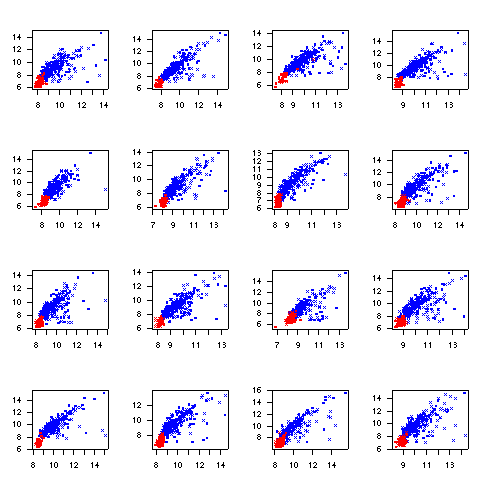
\includegraphics{gridcheck.png}
\caption{Grid check plot for the first array in kidney data}
\label{fig:gridcheck}
\end{figure}
\begin{Sinput}
R> riplot(kidney.raw)
\end{Sinput}
\Rfunction{riplot} stands for ratio-intensity plot. It is also called MA plot. 
The riplot for the first array is shown in figure \ref{fig:riplot}. 
\begin{figure}[htbp]
\centering
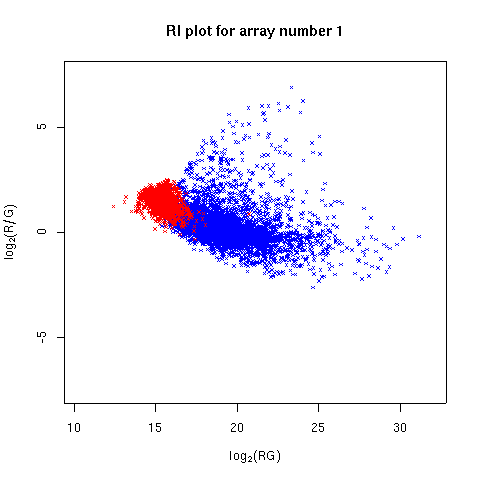
\includegraphics{riplot.png}
\caption{RI plot for the first array in kidney data}
\label{fig:riplot}
\end{figure}
\begin{Sinput}
R> arrayview(kidney.raw)
\end{Sinput}
\Rfunction{arrayview} is used to view the spatial pattern of the arrays.
The standardized log ratios for all spots are shown in different colors.
The arrayview for the first array is shown in figure \ref{fig:arrayview}.
\begin{figure}[htbp]
\centering
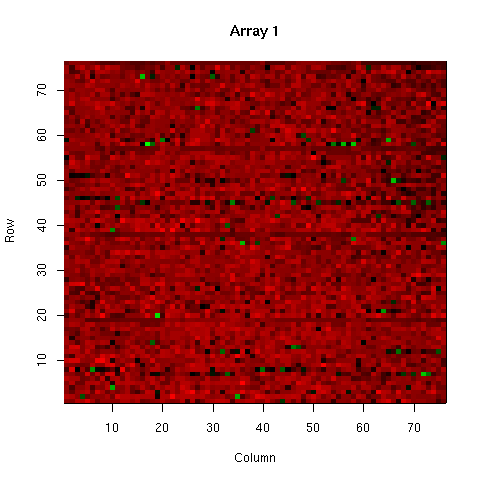
\includegraphics{arrayview.png}
\caption{arrayview for the first array in kidney data}
\label{fig:arrayview}
\end{figure}

You will generate a lot of figures by doing 
gridcheck, riplot and arrayview. Use
\Rfunction{graphics.off} to close all figures.

\item Now make an object of class \Rfunction{madata}.
\Rfunction{madata} and \Rfunction{mamodel}
are the key objects in {\em R/maanova}. Most of the functions work on
them. A \Rfunction{madata} object stores the experimental data. It derived
from the raw data. The \Rfunction{mamodel} object stores the experimental 
design information. We will discuss it a little later.
\begin{Sinput}
R> kidney <- createData(kidney.raw)
R> summary(kidney)
\end{Sinput}

\item Transform the data using spatial-intensity joint loess.
\begin{Sinput}
R> kidney <- transformMadata(kidney, method="rlowess")
\end{Sinput}

There are several data transformation method. Which method to use depends on
the data. Read Cui {\it et al.}(2002) for detail. The transformation
plot for the first array is shown in figure \ref{fig:lowess}.

\begin{figure}[htbp]
\centering
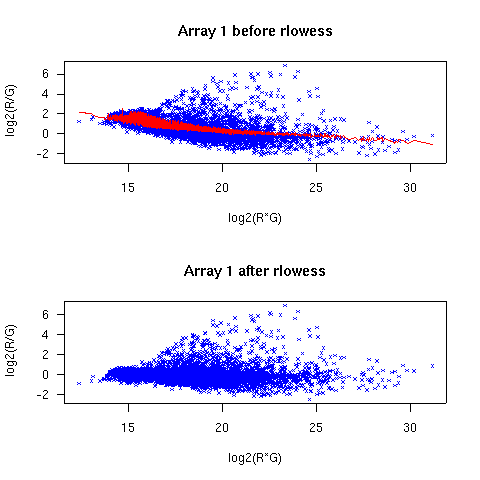
\includegraphics{rlowess.png}
\caption{Joint lowess transformation on the first array for the kidney data}
\label{fig:lowess}
\end{figure}

\item Make model object for fixed model
\begin{Sinput}
R> model.fix <- makeModel(data=kidney, formula=~Dye+Array+Sample)
R> summary(model.fix)
\end{Sinput}

A \Rfunction{mamodel} object store the experimental design information. 
\Rfunction{makeModel} function takes a data object and a R formula as
the ANOVA model and make the design matrices. The input formula is an object
of \Rfunction{formula}. It represents
the ANOVA model. In the formula, you can put any combination of the factors
in your design. Interaction between any two terms are allowed. At this 
point, 3 or higher way interactions are not taken by the program. 
\Rfunction{makeModel} takes another argument 
\Rfunction{ random} for the random terms.
\Rfunction{random} must be another formula. 
All terms in \Rfunction{random} must
be included in \Rfunction{formula} as well. 

\item Fit ANOVA model and do residual plot
\begin{Sinput}
R> anova.fix <- fitmaanova(kidney, model.fix)
R> resiplot(kidney, anova.fix)
\end{Sinput}

\item Permutation F test. F-test function can test one or multiple
terms in a given model object. User can do residual shuffling or
sample shuffling for fixed effect models. For mixed effects models,
only sample shuffling is available. Permutation test could be very
time consuming, especially for mixed effects models. The permutation
test function can run on linux clusters through message passing 
interface (MPI). For detailed information about F test and 
using computer cluster, please read appendix. 

Here we want to test Sample effect in the model:
\begin{Sinput}
R> test.fix <- matest(kidney, model=model.fix, term="Sample", 
       n.perm=500)
\end{Sinput}

Now \Rfunction{test.fix} contains the tabulated P values and permutaion
P values. Sometimes we want to calculate FDR adjusted P values 
for the test result.
\begin{Sinput}
R> test.fix <- adjPval(test.fix)
\end{Sinput}

After getting the F-test result, We can do volcano plot
to visualize it. \Rfunction{volcano} function has options to 
choose the P-values to use and set up thresholds. We will
use tabulated P values for F1 and FDR adjusted permutation 
P values for other tests here. 
In the plot, the orange dots above the horizontal line represent
the significant genes. 
Note that the the flagged spot can be highlighted in the plot. 
You can turn if on by providing \Rfunction{highlight.flag=TRUE}.
\begin{Sinput}
R> idx.fix <- volcano(test.fix,method=c("unadj", rep("fdrperm",3)),
         highlight.flag=FALSE)
\end{Sinput}

The volcano plot is shown in figure \ref{fig:volcano}.
\begin{figure}[htbp]
\centering
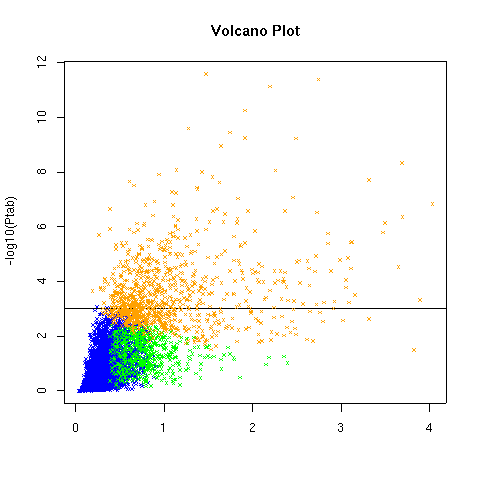
\includegraphics{volcano.png}
\caption{Volcano plot for kidney data - fixed effect model}
\label{fig:volcano}
\end{figure}
Note that the return variable of volcano contains the indices
for significant genes.

\item Now we can do cluster bootstrapping and build consensus trees.
Currently two cluster methods are implemented, hierarchical clustering
and K-means. Hierarchical cluster could be very sensitive to bootstrap
if you have too many leaves on the cluster. 
Some small disturbance on the data could change the whole tree structure. 
So if you have many genes, say, more than 50, and you want to build a
consensus tree from 100 bootstrapped hierarchical trees. It is very
likely that you get a comb, that is, all leaves are directly under 
root. But if you only have a few genes to cluster, it is working fine. 
So I suggest user use K-means to cluster the genes and use hierarchical
to cluster the samples. 

\Rfunction{macluster} is the function to 
do cluster bootstrapping and \Rfunction{consensus}
is used to build consensus trees (groups for K-means) from the 
bootstrap results.
\begin{Sinput}
R> cluster.kmean <- macluster(anova.fix, ,term="Sample",
         idx.gene=idx.fix$idx.all,what="gene", method="kmean"
         kmean.ngroups=5, n.perm=100)
R> con.kmean <- consensus(cluster.kmean, 0.7)
\end{Sinput}
An expression profile plot will be generated for the consensus K-means
result. The plot is shown in figure \ref{fig:vgprofile}.

\begin{figure}
\centering
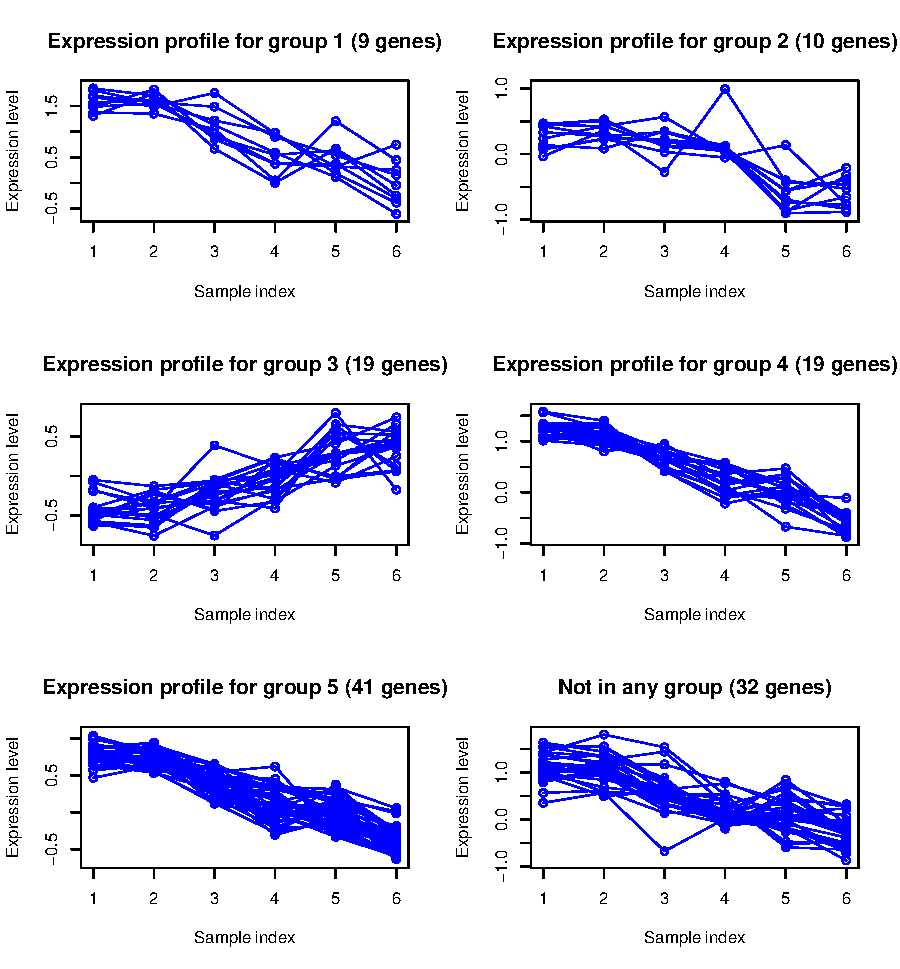
\includegraphics{vgprofile}
\caption{Expression profile plot for bootstrap K-means result, kidney data}
\label{fig:vgprofile}
\end{figure}

Now we can do hierarchical cluster on the samples. The consensus tree 
is shown in figure \ref{fig:hckidney}.
\begin{Sinput}
R> cluster.hc <- macluster(anova.fix, term="Sample",
     idx.gene=idx.fix$idx.all,what="sample", method="hc", n.perm=100)
R> con.hc <- consensus(cluster.hc)
\end{Sinput}

\begin{figure}[htbp]
\centering
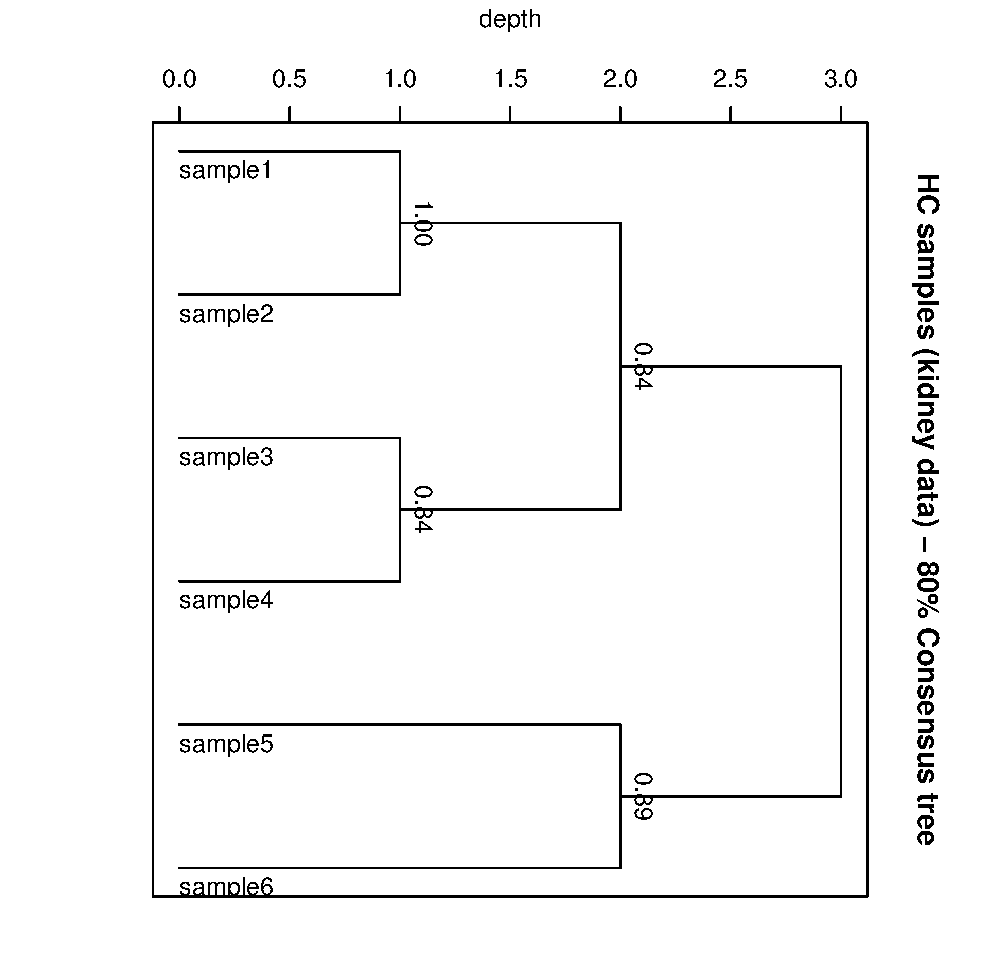
\includegraphics{hckidney}
\caption{80\% Consensus tree for bootstrapping hierarchical cluster on the samples,
kidney data}
\label{fig:hckidney}
\end{figure}

\item Now we are going to analyze the data using mixed effect model. 
First we make a model object with Array effect as random factor. Note 
that normally Array effect, Spot effect and Labeling effect
should be treated as random. Since we don't have technical replicate
here, Spot and Label cannot be fitted.
\begin{Sinput}
R> model.mix <- makeModel(data=kidney, formula=~Dye+Array+Sample, 
           random=~Array)
R> summary(model.mix)
\end{Sinput}

\item Then we can fit the ANOVA model. This will take quite a while to finish.
EM algorithm is implemented in the engine function for solving MME.
For details about MME and the EM algorithms, read Searle {\it et al.}.
\begin{Sinput}
R> anova.mix <- fitmaanova(kidney, model.mix)
\end{Sinput}

\item Now we test the sample effect. Again, permutation test for
mixed effects model is very slow. You have better run it on 
computer clusters if possible.
\begin{Sinput}
R> ftest.mix <- matest(data=kidney, model=model.mix, term="Sample", 
      n.perm=100)
\end{Sinput}
We can do volcano plot for the mixed model result.
\begin{Sinput}
R> idx.mix <- volcano(anova.mix, ftest.mix)
\end{Sinput}

The rest of the analysis (clustering and consensus trees) are skipped here.
\end{enumerate}


